\chapter{Advanced Methods for Attribute Installation in Synthetic Smokers}
\label{ch:synthetic-doppelganger}

As established in the previous chapter, creating personas with arbitrary backstories made it difficult to rigorously assess the \textbf{representativeness} and \textbf{fidelity} of our synthetic agents. To overcome these limitations, we developed the ``doppelgänger'' methodology—a data-driven approach designed to create synthetic twins of actual human participants, enabling a more direct and reliable validation approach.

This method uses a rich dataset from a previous feasibility study on human smokers using MIBot v6.3A (see \Cref{ch:mibot-feasibility-study}), which we refer to by the shorthand \textbf{MIV6.3A}. The dataset contains 106 complete MIBot--human interactions, including demographic data, smoking history (e.g., Heaviness of Smoking Index---HSI), pre- and post-conversation readiness rulers (\emph{importance}, \emph{confidence}, \emph{readiness}), and full conversation transcripts. By extracting and installing attributes directly from this human data, we can create doppelgängers that mirror a real-world distribution. This chapter details the specific methods for creating and evaluating these synthetic doppelgängers.

\section{The Doppelgänger Methodology: A Data-Driven Approach}
\label{sec:synthetic-smoker-doppelgänger}

For the rest of our discussion, we define a doppelgänger as a synthetic smoker designed to be a ``behavioural twin'' of a specific human participant from the feasibility study, although this definition can be extended to other types of participants and studies. The goal is to create an agent that, when exposed to MI counselling, behaves similarly to its human counterpart in terms of language use, psychological profile, and changes in readiness to quit.

Using the doppelgänger methodology provides a straightforward approach to validating the fidelity of synthetic smokers. Rather than using a method $M$ to approximate installed attributes $\hat{\textbf{A}}_S$ from an observation $\gamma_S$, we can devise a reliable and clinically grounded classifier ($\textbf{C}$) that operates on $\gamma$. For example, we can calculate the fraction of change talk (\%CT) from the transcripts.

Further, we can use this classifier to find the distance $d(\textbf{C}(\gamma_H), \textbf{C}(\gamma_S))$. Since, in the case of doppelgängers, $\textbf{A}_S = \textbf{A}_H$, we can approximate the fidelity as:

$$\hat{\mathcal{F}}(\textbf{A}^\textbf{C}) = \mathbb{E}_{\gamma_H \sim P_H (\gamma | \textbf{A}_H),  \:  \gamma_S \sim P_S(\gamma | \textbf{A}_H)}[d(
	\textbf{C}(\gamma_H),\textbf{C}(\gamma_S)
	)]$$


where $\textbf{A}^\textbf{C} = \{a \in \textbf{A} \mid a \sim \textbf{C}(\gamma)\}$. For example, if the correlation between the \%CT of human and synthetic smokers is high, this can approximate the fidelity, $\hat{\mathcal{F}}$. One drawback is that this kind of validation can only measure whether certain attributes are installed and evidenced in the language. It cannot provide a complete picture of fidelity across all attributes. Hence, it approximates the fidelity over a small subset of attributes, $\textbf{A}^\textbf{C}$, i.e., those attributes that are discernible by the classifier $\textbf{C}(\gamma)$.



\section{The Conversational Impact Modelling Experiment}
\label{sec:transcript-autoplay}

Before attempting to install attributes in doppelgängers and have them engage in novel conversations with MIBot, we needed to establish a baseline understanding of the LLM's ability to model the psychological effect of a conversation and contextualize numerical readiness rulers with other installed attributes. For this purpose, we designed the ``Conversational Impact Modelling'' experiment to determine if an LLM-based synthetic smoker (a doppelgänger), when given the pre-conversation attributes of a human participant and the exact transcript of the MIBot--human conversation, can accurately report the same post-conversation readiness rulers as the human.

\subsubsection{Methodology}
\begin{enumerate}
	\item Install the pre-conversation attributes of a specific human participant in the doppelgänger.
	\item Feed the transcript of the actual conversation sequentially to the doppelgänger, framing it as a dialogue in which the doppelgänger is participating.
	\item After the conversation concludes, ask the doppelgänger to complete the post-conversation readiness rulers.
\end{enumerate}

In other words, the doppelgänger was provided with the participant's actual pre-conversation readiness rulers (importance, confidence, and readiness) and the full transcript of their conversation with MIBot. After processing this information, the doppelgänger was asked to report its post-conversation readiness rulers.

The doppelgänger was given the system prompt detailed in \Cref{app:doppelganger-prompts}. An excerpt is shown below:

\includesystemprompt{Conversational Impact Modelling Prompt}{
	You are a participant in a study who is trying to quit smoking.\\
	Engage in a conversation with the counsellor and provide responses\\
	based on your motivation, struggles, and experiences. Your assistant\\
	role is the client, and the user's role is the counsellor or\\
	the researcher.\\\\
	Before you talk to the counsellor, please answer the following
	questions. \\\\
	\quad On a scale from 0 to 10, how important is it to you right\\
	now to stop smoking? Respond with a single integer between 0 (very\\
	low importance) and 10 (very high importance).\\\\
	...
}

To investigate the doppelgänger's reasoning process and potentially improve its accuracy, we used several prompting techniques:

\begin{enumerate}
	\item \textbf{Baseline:} A standard prompt asking the doppelgänger for the post-conversation score.
	\item \textbf{Chain-of-Thought (CoT):} An improved prompt that required the doppelgänger to articulate its reasoning by reflecting on the conversation's key insights, its own motivations, and any expressed shifts in perspective before providing the final numerical score.
\end{enumerate}

We tested this methodology with multiple underlying models, including GPT-4o and Claude 3.7 Sonnet. For the Claude model, we also used its native ``thinking'' feature, which allows the doppelgänger to perform an internal monologue and reflection before generating a final answer, serving as a functional alternative to an explicit CoT prompt.

\subsubsection{Evaluation}
The primary evaluation metrics were the Mean Absolute Error (MAE), Mean Squared Error (MSE), and Spearman's correlation ($r$) between the human-reported and doppelgänger-reported outcomes.

\subsubsection{Results}
First, to establish a performance benchmark, a simple linear regression model was created to predict post-conversation confidence using only pre-conversation confidence from the human data. This yielded an \textbf{MSE of 3.2}, representing the baseline accuracy achievable without considering the conversational content.

The Conversational Impact Modelling experiments consistently outperformed this simple baseline, demonstrating the doppelgänger's ability to extract meaningful signals from the conversation transcripts. An initial ablation study, summarized in \Cref{tab:ablation_results}, reveals the importance of providing the doppelgänger with both the pre-conversation context and the transcript.



\begin{table}[ht!]
	\centering
	\begin{tabular}{@{}lrr@{}}
		\cmidrule(r){1-2}
		\textbf{Input Provided to GPT-4o}                                        & \textbf{Mean Squared Error (MSE)} & \\
		\cmidrule(r){1-2}
		Transcript only                                                          & 5.5                               & \\
		Pre-Conversation Confidence only                                         & 3.7                               & \\
		\textcolor{gray}{Linear Regression (Pre-Conf. $\rightarrow$ Post-Conf.)} & \textcolor{gray}{3.2}             & \\
		Pre-Conversation Confidence + Transcript                                 & 3.1                               & \\
		\textbf{Full Pre-Conversation Rulers + Transcript}                       & \textbf{2.9}                      & \\
		\cmidrule(r){1-2}
	\end{tabular}
	\caption[Ablation study on doppelgängers' self-reported post-conversation confidence]{Impact of different attributes on GPT-4o-based doppelgängers' self-reported post-conversation confidence. Both the pre-conversation readiness rulers and the conversation transcript are necessary for the doppelgängers to accurately report post-conversation confidence. The linear regression model serves as a baseline.}
	\label{tab:ablation_results}
\end{table}



While metrics like MAE provide a quantitative summary, a visual comparison of the distributions reveals some discrepancies. \Cref{fig:post_conf_distributions} plots the distribution of human-reported confidence scores alongside the distribution of GPT-4o-based doppelgänger. Both distributions are similarly left-skewed, indicating that the model correctly identifies that most participants land in the higher-confidence range (6--10). However, the doppelgänger predictions were less varied than the human responses. The human data shows a broader plateau of high confidence across scores of 6, 7, and 8, whereas the doppelgängers exhibit a pronounced peak at a score of 7. This suggests that while the model is effective at capturing the overall positive trend, it may be less sensitive to the subtle individual differences in participants' final confidence levels, tending to revert to a more common or ``average'' high-confidence outcome.



\begin{figure}[ht!]
	\centering
	\begin{minipage}{0.48\textwidth}
		\centering
		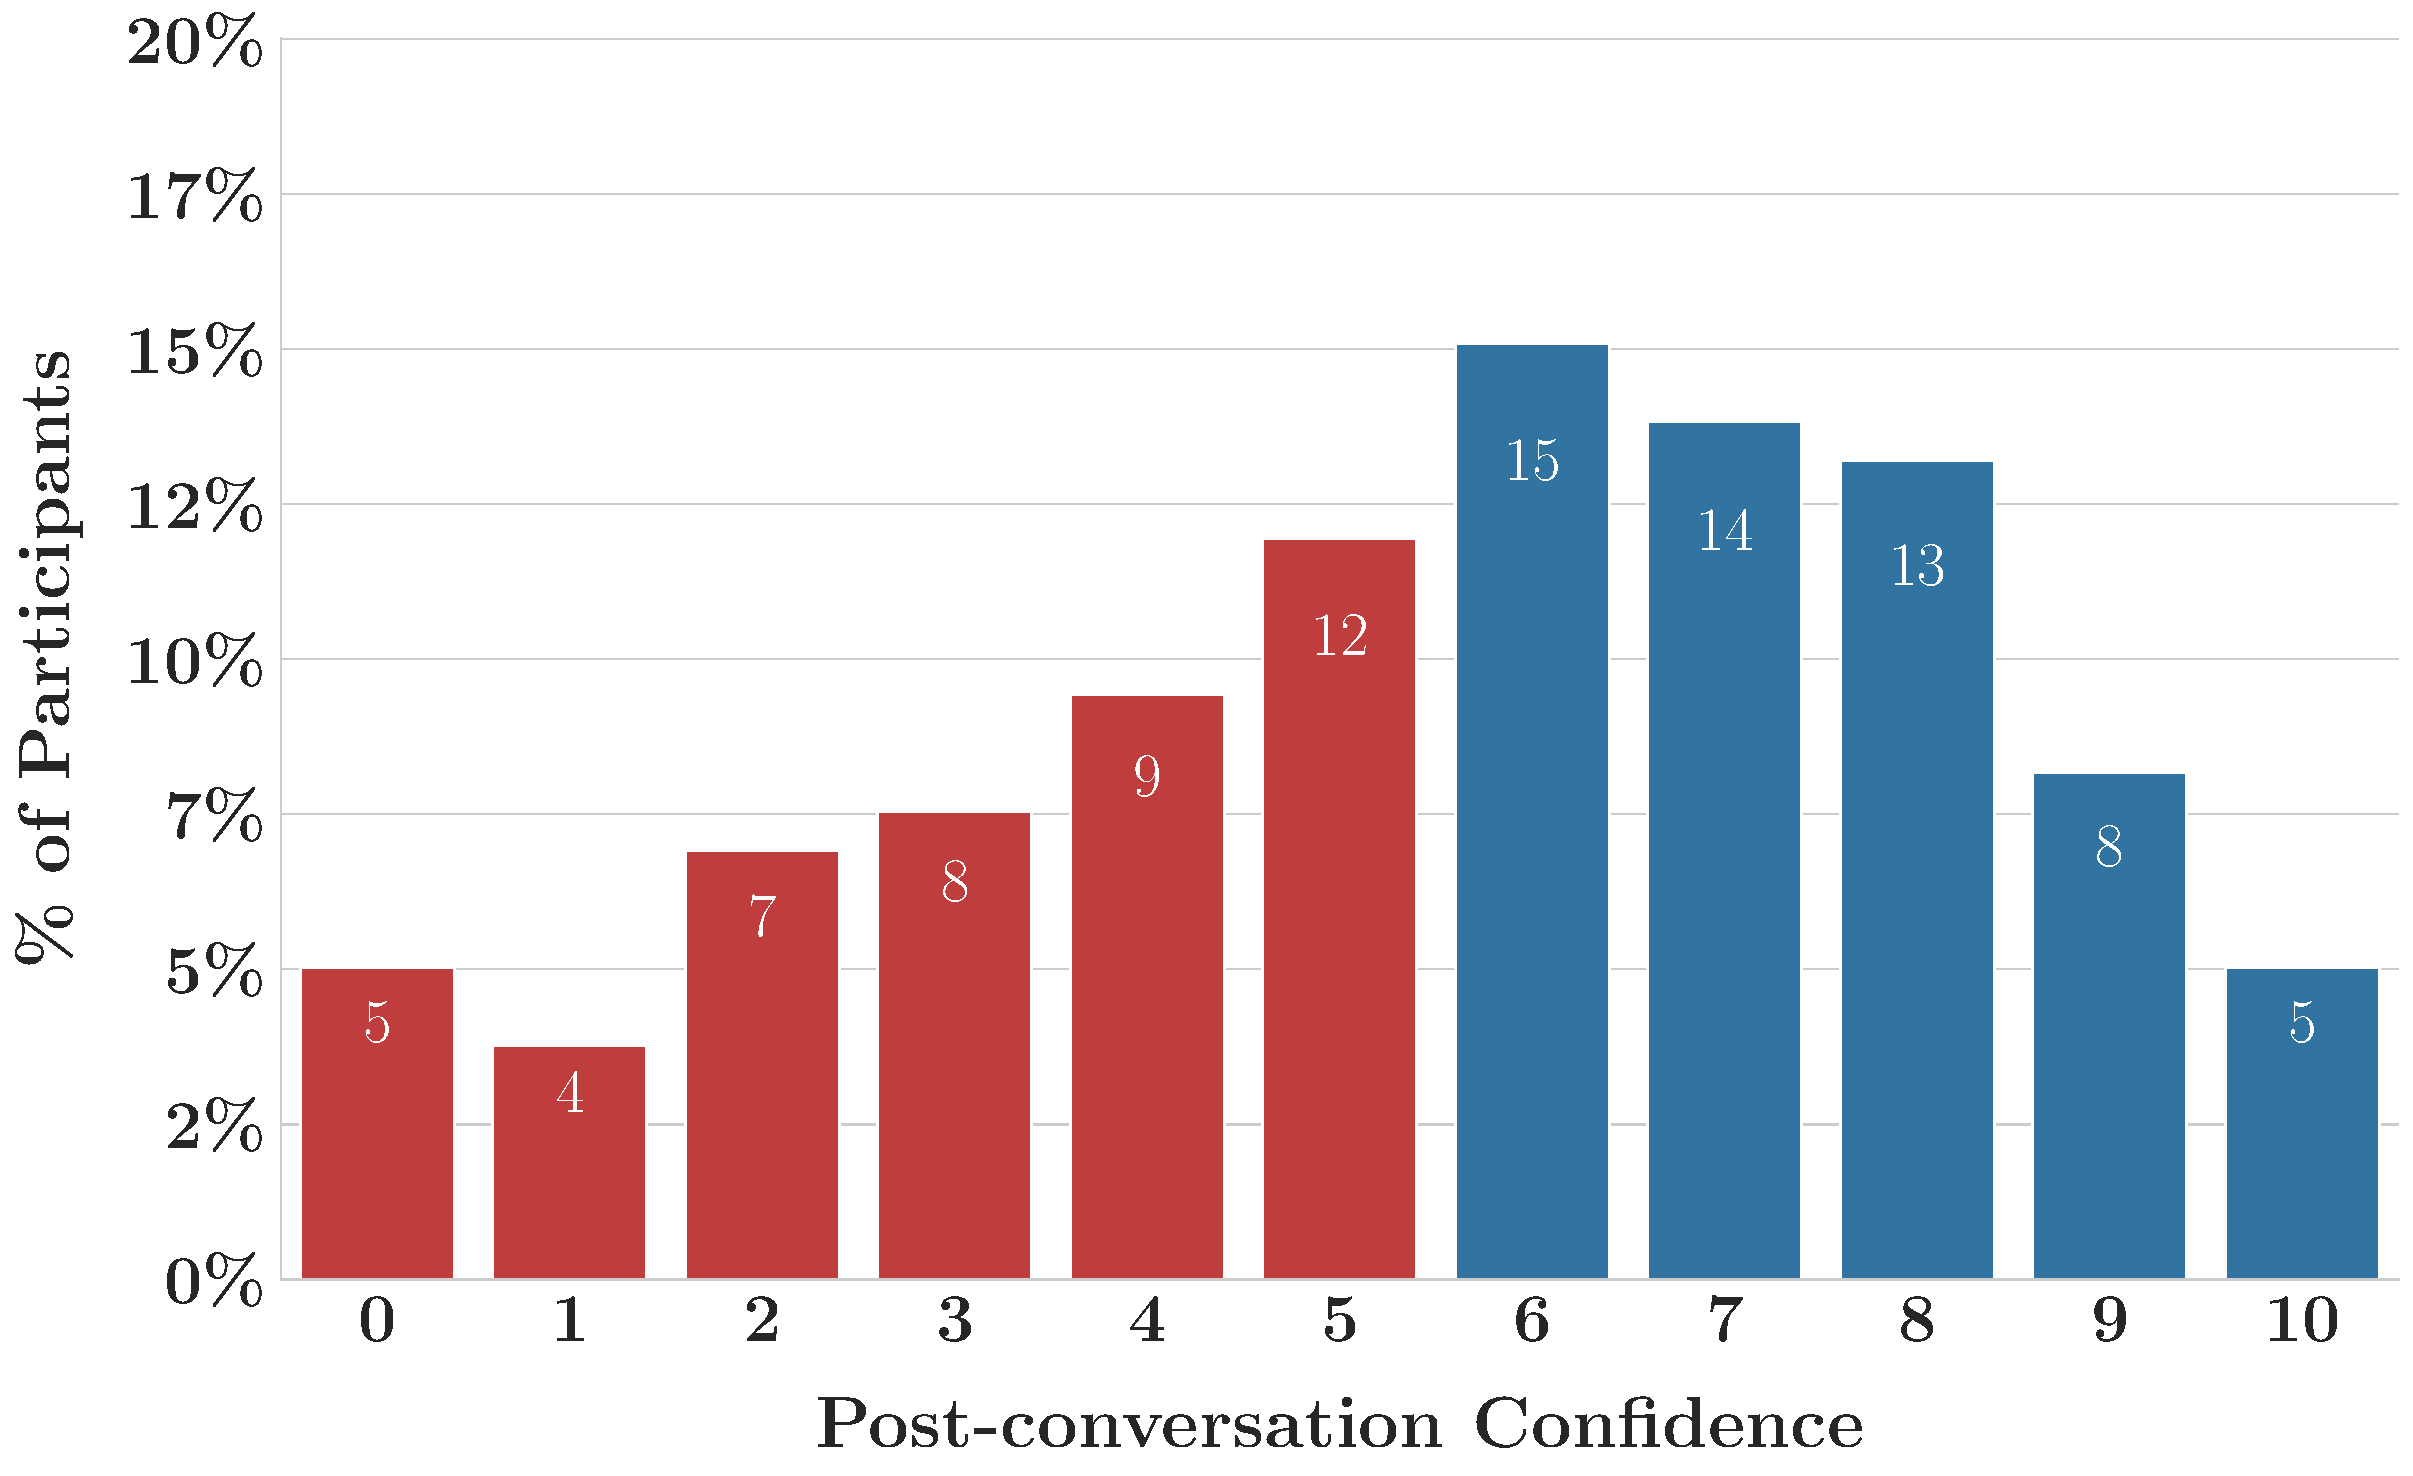
\includegraphics[width=\linewidth]{fig/post-conf-human.pdf}
		\subcaption{Human-reported post-conversation confidence scores}
		% No sub-caption needed as the main caption explains it
	\end{minipage}\hfill
	\begin{minipage}{0.49\textwidth}
		\centering
		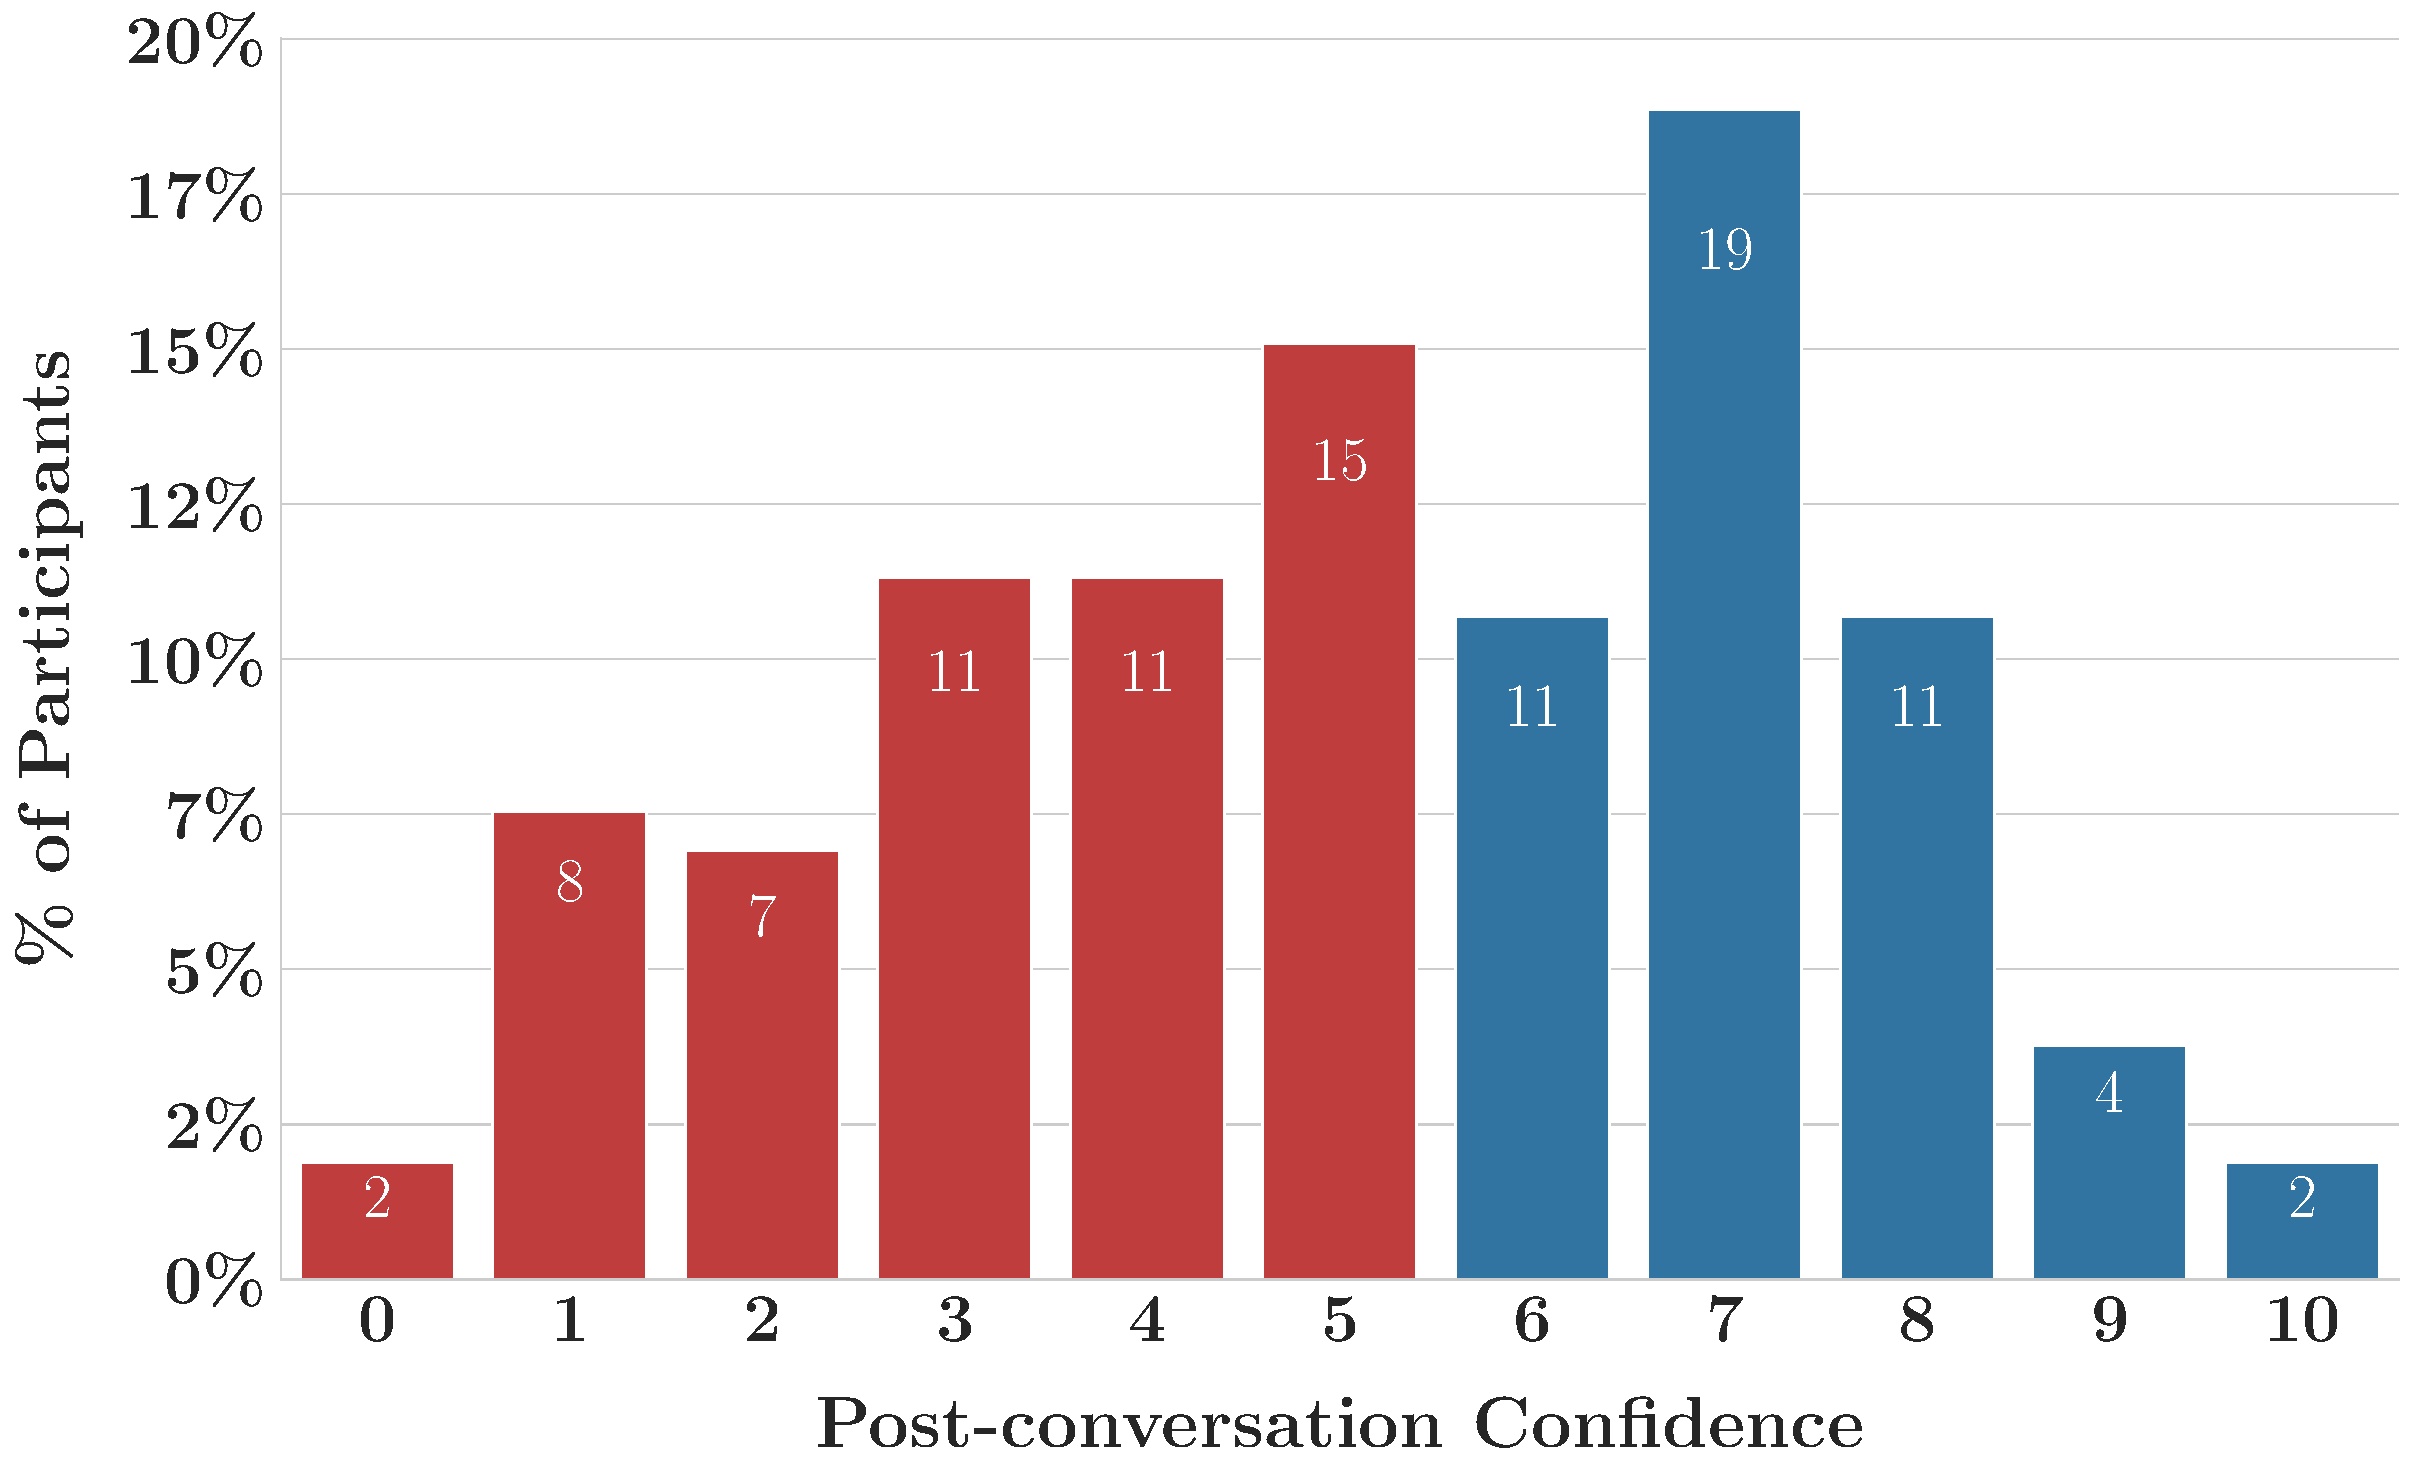
\includegraphics[width=\linewidth]{fig/post-conf-gpt4-o.pdf}
		\subcaption{Doppelgänger-reported post-conversation confidence scores}
	\end{minipage}
	\caption[Distribution of post-conversation confidence scores for humans compared to doppelgängers]{Distribution of post-conversation confidence scores for humans compared to doppelgängers. While the overall shapes are similar, the doppelgänger's scores are more concentrated around a single peak (score of 7), whereas human responses are more distributed across several high-confidence values.}
	\label{fig:post_conf_distributions}
\end{figure}


Next, we compared the performance of different underlying models and prompting techniques used by the doppelgängers to report post-conversation confidence. The results, detailed in \Cref{tab:model_comparison}, show that reflective prompting methods consistently improved accuracy.


\begin{table}[!ht]
	\centering
	\begin{tabular}{l|cccc}
		\toprule
		\textbf{Model}                        & \textbf{MAE} & \textbf{MSE} & \textbf{Correlation ($r$)} & \textbf{Exact Matches (\%)} \\
		\midrule
		GPT-4o (Baseline)                     & 1.2          & 3.0          & 0.7                        & 31
		\\
		GPT-4o (CoT)                          & 1.2          & 2.9          & 0.7                        & 30                          \\
		Claude 3.7 Sonnet (CoT)               & 1.2          & 2.7          & 0.7                        & 31                          \\
		\textbf{Claude 3.7 Sonnet (Thinking)} & \textbf{1.1} & \textbf{2.6} & \textbf{0.8}               & \textbf{32}                 \\
		\bottomrule
	\end{tabular}
	\caption[Effect of LLM type and reasoning on synthetic smokers' self-reported confidence]{Comparison of different models and prompting techniques and their impact on the self-reporting of post-conversation confidence (N=159). Reflective techniques, especially Claude 3.7 Sonnet's ``thinking'' feature, yielded the best results across all metrics.}
	\label{tab:model_comparison}
\end{table}

The baseline GPT-4o doppelgänger achieved a strong correlation of \textbf{$r=0.7$} with the human-reported scores. However, the \textbf{Claude 3.7 Sonnet doppelgänger using its ``thinking'' feature achieved the lowest error (MAE=1.1, MSE=2.6) and the highest correlation ($r=0.8$)}.


\begin{figure}[htpb]
	\centering
	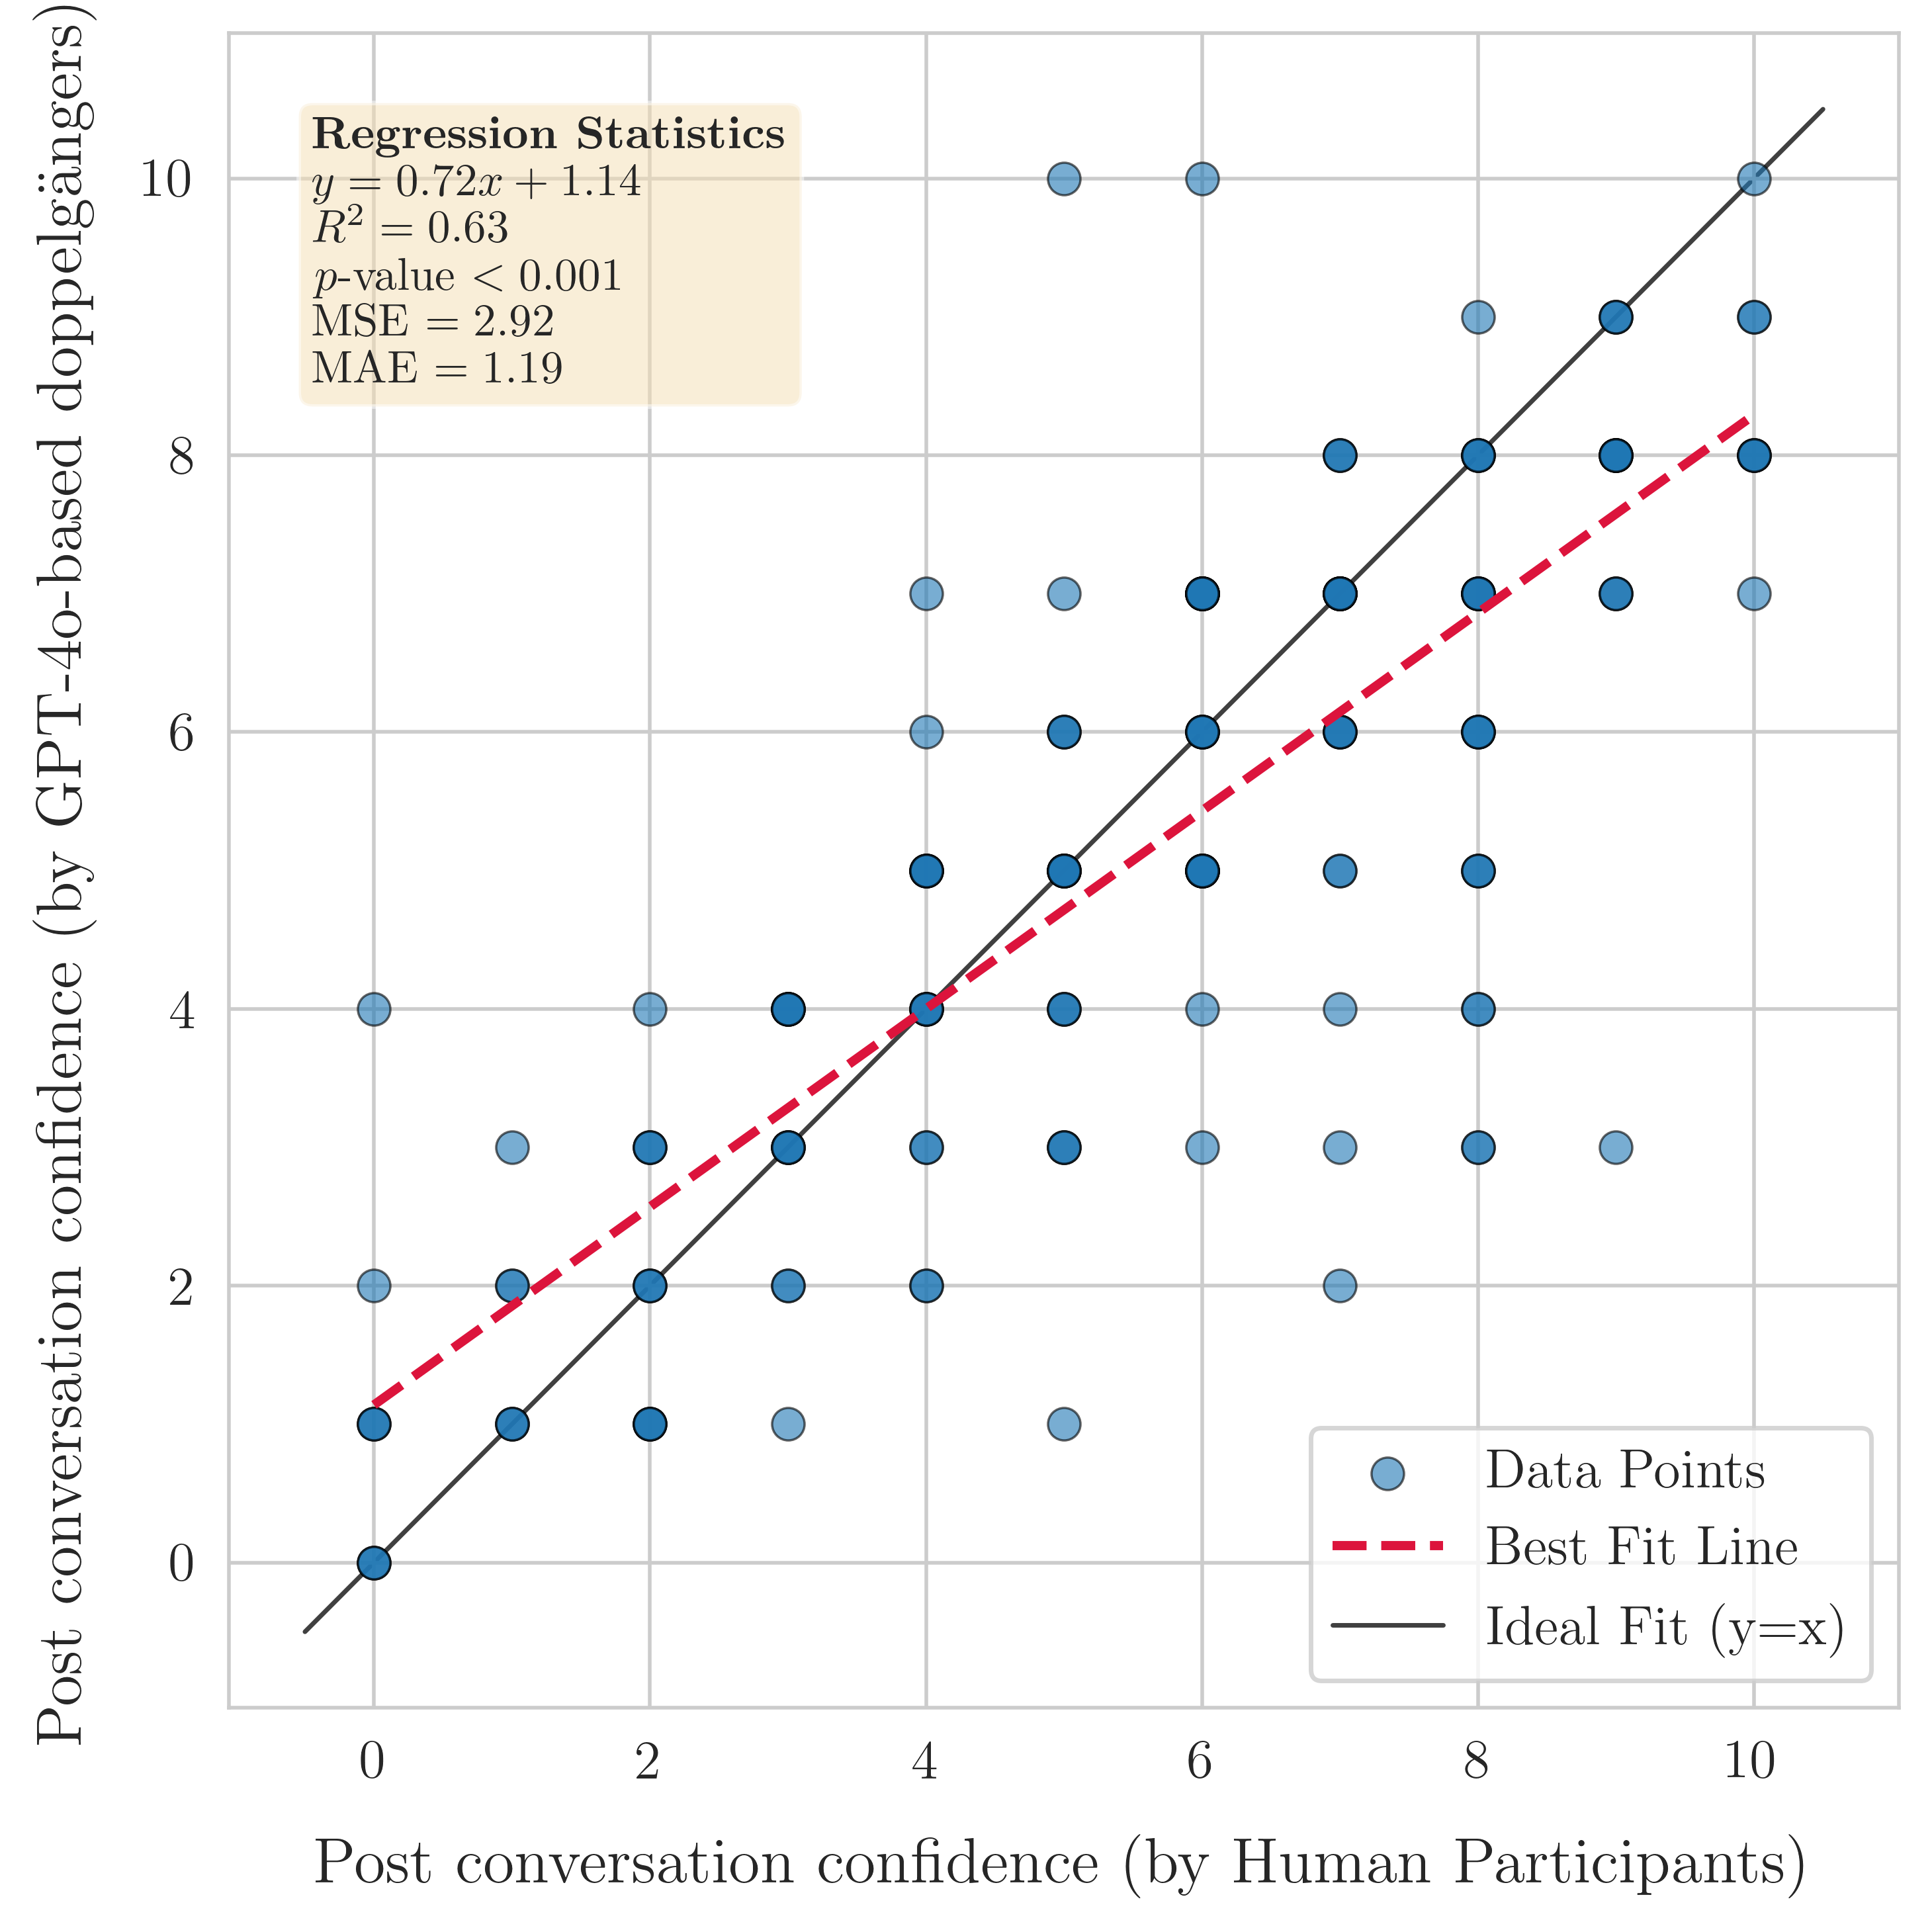
\includegraphics[width=0.5\textwidth]{fig/post_conf_gpt4o_vs_human.png}
	\caption[Scatter plot of human-reported vs. doppelgänger-reported post-conversation confidence]{Scatter plot of human-reported vs. doppelgänger-reported post-conversation confidence for the baseline GPT-4o model, showing a Spearman's correlation of r=0.70. The diagonal line represents perfect agreement.}
	\label{fig:post-conf-gpt4o-vs-human}
\end{figure}


\Cref{fig:post-conf-gpt4o-vs-human} visualizes the relationship between the post-conversation confidence reported by human participants and that reported by their corresponding GPT-4o-based doppelgängers. The analysis reveals a strong, statistically significant positive correlation (Spearman's $r=0.70, p < 0.001$), indicating that the doppelgängers are generally successful in mirroring the human outcomes after processing the conversation transcript. The Mean Absolute Error (MAE) was 1.19, suggesting the doppelgänger's reported score was typically within about 1.2 points of the human's score on the 0--10 scale.

However, the plot also reveals a notable trend when comparing the best-fit line (dashed red) with the ideal fit (solid black). The regression equation ($y=0.72x+1.14$) shows a slope less than 1.0 and a positive intercept. This indicates a tendency towards ``regression to the mean'' in the doppelgänger reports. Specifically, when human participants reported very low confidence (e.g., 0--3), the doppelgängers tended to report slightly higher confidence (closer to the intercept of 1.14). Conversely, when humans reported very high confidence (e.g., 8--10), the doppelgängers tended to report slightly lower confidence. This suggests that while the directional impact of the conversation is captured well, the magnitude of the impact at the extremes might be slightly attenuated in the synthetic agents.

We further extended this analysis to include the other two readiness rulers: importance and readiness. The results are summarized in \Cref{tab:autoplay_results_full}.




\begin{table}[!ht]
	\centering
	\begin{tabular}{l|cc|cc|cc}
		\toprule
		                      & \multicolumn{2}{c|}{\textbf{Post-Confidence}} & \multicolumn{2}{c|}{\textbf{Post-Importance}} & \multicolumn{2}{c}{\textbf{Post-Readiness}}                                                  \\
		\textbf{Model}        & \textbf{MAE}                                  & \textbf{Corr.}                                & \textbf{MAE}                                & \textbf{Corr.} & \textbf{MAE} & \textbf{Corr.} \\
		\midrule
		GPT-4o (CoT)          & 1.2                                           & 0.7                                           & 0.8                                         & 0.9            & 0.7          & 0.9            \\
		Claude 3.7 (Thinking) & 1.1                                           & 0.8                                           & 0.7                                         & 0.9            & 0.9          & 0.8            \\ \hline
	\end{tabular}
	\caption[Multi-ruler conversational impact modelling results]{Results of the conversational impact modelling experiment across all three readiness rulers, showing MAE and Pearson correlation. Performance was consistently strong, especially for importance and readiness.}
	\label{tab:autoplay_results_full}
\end{table}

\Cref{tab:autoplay_results_full} summarizes the performance of the Conversational Impact Modelling experiment across all three readiness rulers. The results demonstrate high correlations (ranging from 0.7 to 0.9) across all rulers for both GPT-4o and Claude 3.7 models, affirming the robustness of the methodology.

It is interesting to note that the performance metrics for post-importance and post-readiness are generally stronger than for post-confidence. For example, the correlations for importance (0.9 for both models) are notably higher, and the MAEs are lower than for confidence. This suggests that the doppelgängers found it easier to accurately model the conversational impact on a participant's sense of importance and readiness to quit than on their self-efficacy (confidence) in their ability to do so. Overall, the Claude 3.7 model utilizing its ``thinking'' feature demonstrated slightly better performance in modelling confidence (correlation 0.8, MAE 1.1) compared to GPT-4o (correlation 0.7, MAE 1.2).



This experiment served as a check on the doppelgänger's ability to infer the psychological state resulting from the conversation. The underlying model possesses the necessary reasoning capabilities to allow the doppelgänger to understand how conversational dynamics influenced the participant's motivation and confidence. This serves as a baseline to confirm the doppelgänger's internal consistency before attempting to generate the conversation itself.



\section{Experiments with the Incremental Installation of Attributes}
Having gained insights into the LLM's ability to model conversations and its intuitive understanding of numerical attributes such as readiness rulers, we set out to systematically install attributes in LLM-based synthetic smokers and validate their installation. Recall from our discussion on the benefits of creating doppelgängers (\Cref{sec:synthetic-smoker-doppelgänger}). They provide a way to approximate the fidelity of an installation and make the validation of synthetic agents easier. We can approximate the fidelity of synthetic smokers with the correlation between some metric on the observable outer space (e.g., transcripts) of doppelgängers and their human twins. As an example, to validate whether the behavioural attribute of resistance to change has been successfully installed, we can analyze the transcripts from both humans and their doppelgängers and calculate the correlation between the percentage of Change Talk (\%CT) exhibited by both groups. A high correlation would then suggest a successful installation of this attribute.


\subsection*{Percentage Change Talk: A Key Metric for Validating Behavioural Fidelity}

To validate the synthetic smokers developed using the doppelgänger method, we needed an objective metric that could measure the smokers' level of motivation from their language.
We identified the percentage change talk metric (also referred to as change fraction or CF, calculated as CT / (CT + ST)) to fit our requirements, as it is grounded in the client's language and is strongly associated with behavioural change outcomes in MI~\cite{Barnett2014,Houck2018,Moyers2009,Baer2008}.
Furthermore, we tested if \%CT is a valid proxy for a client's internal state, i.e., if it correlates with established metrics of readiness in human participants.

We analyzed the data from MIV6.3A ($N=106$ participants). The analysis confirmed strong, statistically significant correlations between \%CT and all readiness rulers (\Cref{tab:ct-correlation}). For example, the correlation with post-conversation confidence was 0.41 ($p < 0.0001$). These results motivated us to use \%CT as a primary metric for validating the installation of behavioural attributes in the synthetic smoker.


\begin{table}[!ht]
	\centering
	\begin{tabular}{@{}lr@{}}
		\toprule
		\textbf{Attribute}               & \textbf{Correlation with \%CT} \\
		\midrule
		Pre-conversation importance      & 0.47$^{****}$                  \\
		Pre-conversation confidence      & 0.29$^{**}$                    \\
		Pre-conversation readiness       & 0.46$^{****}$                  \\
		\midrule
		Post-conversation importance     & 0.49$^{****}$                  \\
		Post-conversation confidence     & 0.41$^{****}$                  \\
		Post-conversation readiness      & 0.48$^{****}$                  \\
		\midrule
		Change in importance (Post--Pre) & 0.12                           \\
		Change in confidence (Post--Pre) & 0.24$^{**}$                    \\
		Change in readiness (Post--Pre)  & 0.06                           \\
		\midrule
		CARE (perceived empathy)         & 0.15                           \\
		Previous number of quit attempts & 0.09                           \\
		Age                              & -0.11                          \\
		Number of cigarettes per day     & -0.04                          \\
		HSI (Heaviness of Smoking Index) & -0.15                          \\
		\bottomrule
		\multicolumn{2}{l}{\footnotesize{**** $p < 0.0001$, *** $p < 0.001$, ** $p < 0.01$, * $p < 0.05$}.}
	\end{tabular}
	\caption{Correlation between \%CT and human smoker attributes in the MIBot dataset}
	\label{tab:ct-correlation}
\end{table}



\subsection{Methodology}
The doppelgänger methodology uses a dataset of installable human attributes (e.g., MIV6.3A, containing attributes of human smokers) to build and validate synthetic smokers. The process involves:

\begin{enumerate}
	\item \textbf{Attribute Installation:} Instantiating a synthetic smoker, $S_i$, by installing the known attributes of a specific human participant, $H_i$, from the dataset. $A_S = A_H$. These attributes may include demographics, HSI, self-reported survey responses, etc.
	\item \textbf{Simulation:} The synthetic smoker, $S(A_H)$, interacts with the same counsellor (MIBot, in our case) that the original human interacted with.
	\item \textbf{Comparison:} The output of the synthetic smoker, $\gamma_S$, is compared with the actual output of the human, $\gamma_H$ (see \Cref{sec:synthetic-smoker-doppelgänger}).
\end{enumerate}



The overall workflow for creating and validating doppelgängers using this comparative method is illustrated in \Cref{fig:doppelgänger-creation-process}.



We created a set of doppelgängers (N=20) by sampling 20 human participants from MIV6.3A. Then, we conducted a series of experiments on these doppelgängers. In each experiment, we installed a subset of attributes in the doppelgängers via \emph{prompting} and did not add any backstories to their prompt.

\includesystemprompt{Example of attribute installation in doppelgänger prompts}{
	You are a participant in a study who is trying to quit smoking. Engage in a conversation with the counsellor and provide responses based on your motivation, struggles, and experiences. Your assistant role is the client, and the user's role is the counsellor or the \\ researcher. Always try to respond in fewer than 200 characters. \\\\
	About you: You are a 30-year-old female. You typically smoke 25 cigarettes per day. After you wake up, you smoke your first cigarette within 5 minutes. In the past week, you have not made any quit attempts.\\\\
	Before speaking to the counsellor, you have rated your motivation to quit as follows (on a scale from 0 to 10): Importance: 2, Confidence: 0, Readiness: 4. \\\\
	You talk about changing your smoking behaviour 46\% of the time.
	...
}


Before starting our series of experiments, we sorted the set of all installable attributes based on their correlation with \%CT. We hypothesized that a high correlation between an attribute and \%CT would mean that the attribute has a bigger impact on the client's behavioural language. Let us call this sorted list of attributes $\mathbf{A'}$.

$$
	\begin{aligned}
		{\textbf{A}}^{'} = \{ & \text{pre-conversation importance,} \\
		                      & \text{pre-conversation readiness,}  \\
		                      & \text{age,}                         \\
		                      & \text{sex,}                         \\
		                      & \text{pre-conversation confidence,} \\
		\cdots \}
	\end{aligned}
$$

The experiment then proceeds by incrementally adding attributes from this sorted list and, at each step, measuring the fidelity of the resulting doppelgängers. Fidelity is operationalized as the correlation between the percentage change talk (\%CT) of the human participants and their corresponding doppelgängers. The process is detailed in \Cref{alg:incremental_installation}.


The overall workflow for creating and validating doppelgängers using this comparative method is illustrated in \Cref{fig:doppelgänger-study}.

\begin{figure}[htpb]
	\centering
	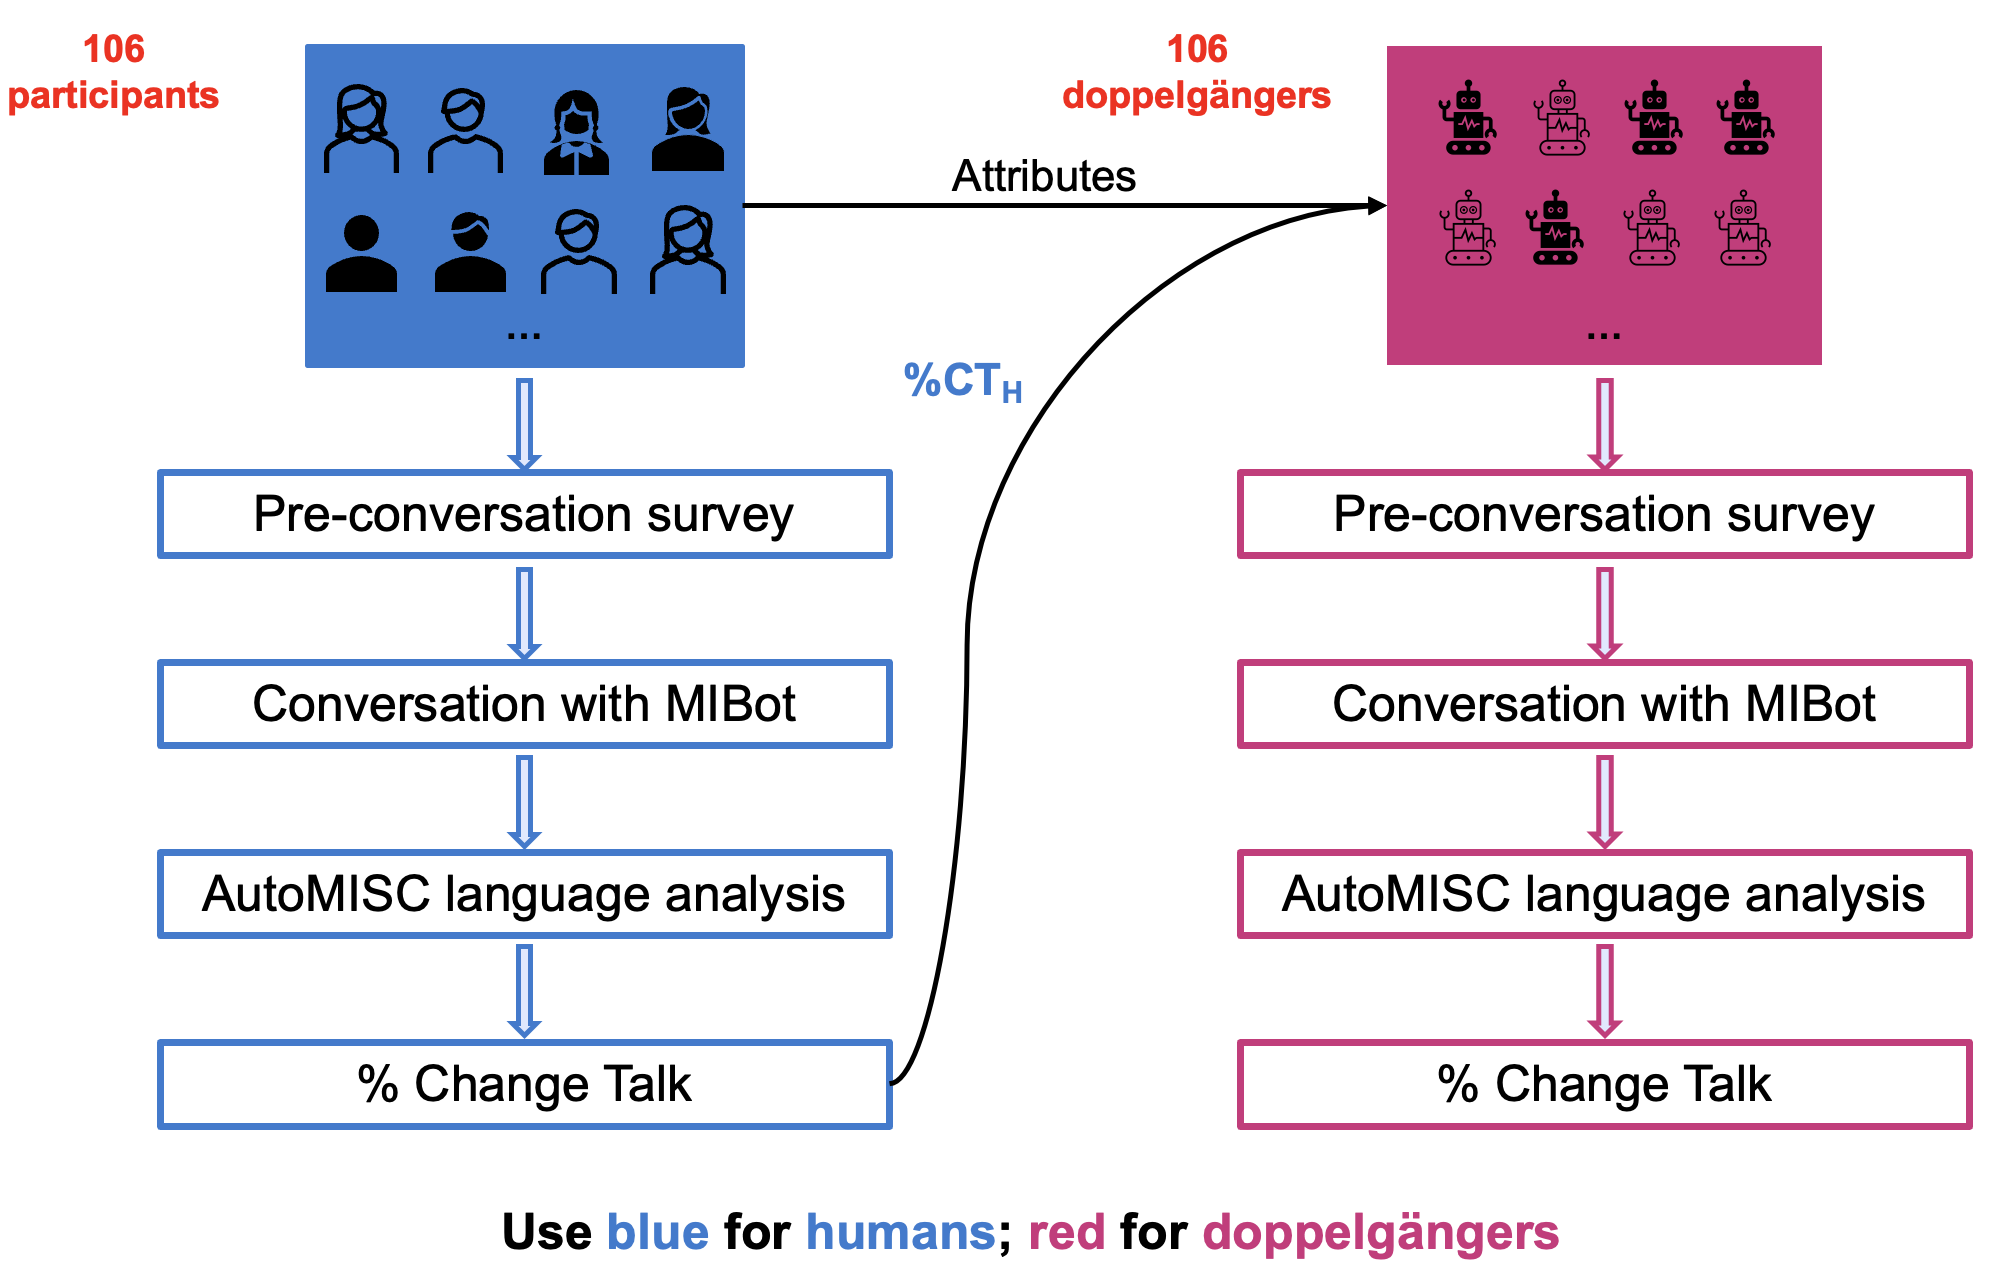
\includegraphics[width=0.98\textwidth]{fig/doppelganger-study.png}
	\caption[Doppelgänger creation and validation process]{Doppelgänger creation and validation process. For each of the 106 human participants ($H_i$), a synthetic twin ($S_i$) is created by installing their attributes. Both agents' conversations with MIBot are analyzed to extract a behavioural metric (\%CT), and the correlation between the two sets of metrics is used to assess fidelity.}
	\label{fig:doppelgänger-study}
\end{figure}

{
\setstretch{1.25}
\begin{algorithm}[htpb]
	\caption{Incremental attribute installation and fidelity validation}
	\label{alg:incremental_installation}
	\begin{algorithmic}[1]
		\Require Human dataset $\mathcal{D} = \{ (H_i, \mathbf{A}_{H_i}, \gamma_{H_i}) \}_{i=1}^N$ containing human participants, their full attribute vectors, and conversation transcripts.
		\Require Sorted list of attributes $\mathbf{A'} = (a'_1, a'_2, \dots, a'_m)$ ordered by hypothesized relevance.\vspace{5pt}
		\State Initialize $\mathbf{A}_{\text{installed}} \leftarrow \emptyset$ \Comment{The set of attributes to install}
		\State Initialize $C \leftarrow ()$ \Comment{An empty list to store correlation results}

		\For{$k \leftarrow 1 \text{ to } m$} \Comment{Iterate through the sorted list of attributes}
		\State $\mathbf{A}_{\text{installed}} \leftarrow \mathbf{A}_{\text{installed}} \cup \{a'_k\}$ \Comment{Add the next attribute}

		\State Initialize $\mathbf{V}_{\text{human\_CT}} \leftarrow ()$ and $\mathbf{V}_{\text{synth\_CT}} \leftarrow ()$ \Comment{Vectors for \%CT scores}

		\For{$i \leftarrow 1 \text{ to } N$} \Comment{For each human participant in the dataset}
		\State $\mathbf{A}_{\text{subset}} \leftarrow \mathbf{A}_{H_i} |_{\mathbf{A}_{\text{installed}}}$ \Comment{Filter attributes for the current iteration}
		\State $S_i \leftarrow \mathcal{S}(\mathbf{A}_{\text{subset}})$ \Comment{Instantiate the synthetic smoker $S_i$ with the given parameters}
		\State Simulate a conversation between $S_i$ and MIBot to generate transcript $\gamma_{S_i}$.

		\State Calculate human \%CT: $c_{H_i} \leftarrow \text{\%CT}(\gamma_{H_i})$
		\State Calculate synthetic \%CT: $c_{S_i} \leftarrow \text{\%CT}(\gamma_{S_i})$

		\State Append $c_{H_i}$ to $\mathbf{V}_{\text{human\_CT}}$
		\State Append $c_{S_i}$ to $\mathbf{V}_{\text{synth\_CT}}$
		\EndFor

		\State Calculate the correlation for the current attribute set: $\rho_k \leftarrow \text{Correlation}(\mathbf{V}_{\text{human\_CT}}, \mathbf{V}_{\text{synth\_CT}})$
		\State Append $\rho_k$ to the results list $C$.
		\EndFor
		\vspace{5pt}
		\State \Return $C$ \Comment{A list of correlations, one for each incremental step of attribute installation}
	\end{algorithmic}
\end{algorithm}
}



\begin{figure}[htpb]
	\centering
	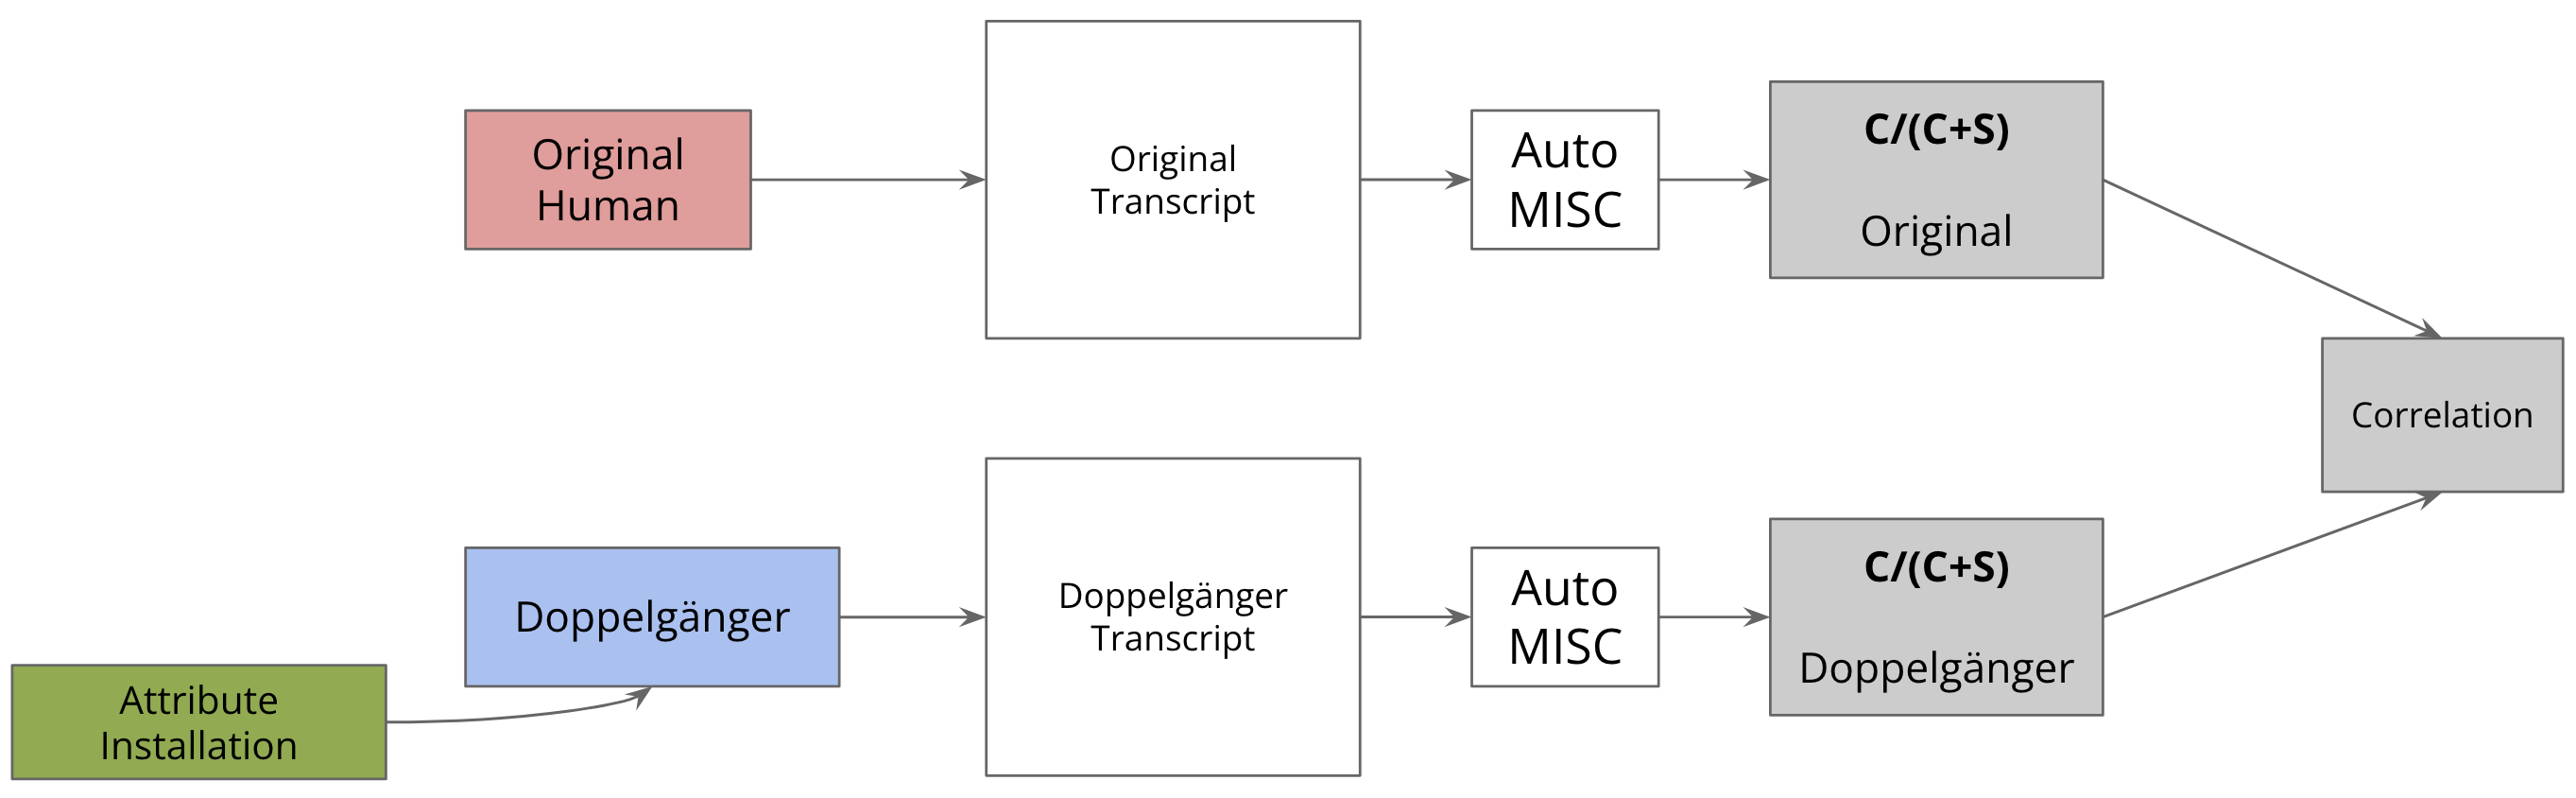
\includegraphics[width=0.98\textwidth]{fig/doppelganger_process.png}
	\caption[Brief overview of doppelgänger creation and validation process]{Brief overview of doppelgänger creation and validation process.}
	\label{fig:doppelgänger-creation-process}
\end{figure}

\subsection{Evaluation}
For each experiment with a set of attributes, we calculated the Spearman's correlation coefficient between the \%CT of human--MIBot and doppelgänger--MIBot conversations.



\subsection{Results}
The results of the incremental attribute installation are summarized in \Cref{tab:doppelgänger-correlations}. The fidelity, measured as the Spearman's rank correlation between the \%CT of humans and their doppelgängers, evolved as more attributes were added. Initially, adding attributes like pre-conversation importance and readiness led to a gradual increase in correlation. However, the process was not strictly monotonic; for instance, adding `pre-conversation confidence' in experiment 5 unexpectedly lowered the correlation from 0.40 to 0.22.

The most significant finding emerged in experiment 6, where explicitly installing the human's \%CT value as a numerical instruction resulted in a strong and statistically significant correlation of $r_s = 0.57$ ($p < 0.0001$). This suggests an LLM-based doppelgänger can directly operationalize a behavioural target when provided, modulating its language to match a specified proportion of change versus sustain talk.

However, despite achieving a strong rank correlation, a closer look at the population-level statistics reveals a systematic bias. As shown in the histograms in \Cref{fig:cf_comparison}, the distribution of \%CT for doppelgängers is shifted significantly higher than for humans (mean 0.76 vs. 0.59). The doppelgänger distribution is also more compressed and left-skewed, indicating a lower variance and a strong tendency to produce high levels of change talk, regardless of the human baseline.

This discrepancy is further visualized in the scatter plot in \Cref{fig:cf_human_vs_doppel}. While the points follow a positive trend that confirms the correlation, the majority lie above the identity line ($y=x$). This visually demonstrates that doppelgängers consistently overproduced change talk relative to their human counterparts. Even when a human participant had a low \%CT (e.g., below 0.4), their doppelgänger often produced a \%CT above 0.6 (see \Cref{app:doppelganger-transcript} for an example transcript).

Finally, we investigated the system's uniform fidelity by stratifying the results by sex, as detailed in \Cref{tab:doppelgänger-fidelity-sex}. While the mean \%CT for both human males and females was nearly identical ($\sim$59\%), the fidelity of their doppelgängers differed. The correlation for males ($r_s = 0.65$) was notably stronger than for females ($r_s = 0.52$), indicating a performance bias. This lack of uniform fidelity suggests the model may simulate one demographic group more accurately than another, an issue requiring further investigation to ensure representative synthetic populations. Other observations include:

\begin{enumerate}
	\item Once an attribute (e.g., pre-conversation importance) is installed in the doppelgängers, it is accurately recalled when prompted.
	\item Asking the doppelgängers to think before filling out the post-conversation readiness rulers reduced the gap (as measured by MAE) between their and human-reported scores.
\end{enumerate}



\begin{table}[ht!]
	\centering
	\begin{threeparttable}
		\sisetup{
			table-format=0.2,
			table-space-text-post = $^{****}$
		}
		\renewcommand{\arraystretch}{1.2}
		\begin{tabular}{c cccccc S}
			\toprule
			\textbf{Experiment} & \multicolumn{6}{c}{\textbf{Installed Attributes}} & {\textbf{\makecell{Spearman's rank                                                                        \\ correlation}}} \\
			\cmidrule(r){2-7}
			                    & \makecell{Pre-conv.                                                                                                                                           \\ importance} & \makecell{Pre-conv. \\ readiness} & Age & Sex & \makecell{Pre-conv. \\ confidence} & \%CT & {$r_s$} \\
			\midrule
			1                   & \checkmark                                        &                                    &            &            &            &            & 0.19             \\
			2                   & \checkmark                                        & \checkmark                         &            &            &            &            & 0.24             \\
			3                   & \checkmark                                        & \checkmark                         & \checkmark &            &            &            & 0.26             \\
			4                   & \checkmark                                        & \checkmark                         & \checkmark & \checkmark &            &            & 0.40             \\
			5                   & \checkmark                                        & \checkmark                         & \checkmark & \checkmark & \checkmark &            & 0.22\tnote{*}    \\
			6                   & \checkmark                                        & \checkmark                         & \checkmark & \checkmark & \checkmark & \checkmark & 0.57\tnote{****} \\
			\bottomrule
		\end{tabular}
		\begin{tablenotes}
			\footnotesize
			\item[*] $p < 0.05$
			\item[**] $p < 0.01$
			\item[***] $p < 0.001$
			\item[****] $p < 0.0001$
		\end{tablenotes}
	\end{threeparttable}
	\caption[Incremental attribute installation and its effect on the fidelity of doppelgängers]{
		Incremental attribute installation and its effect on the fidelity of doppelgängers. Fidelity is measured by the Spearman correlation of percentage change talk (\%CT) between human participants and their doppelgängers (N=20). Each row represents a model where attributes were cumulatively added to the installation prompt.
	}
	\label{tab:doppelgänger-correlations}
\end{table}


\begin{figure}[ht!]
	\centering
	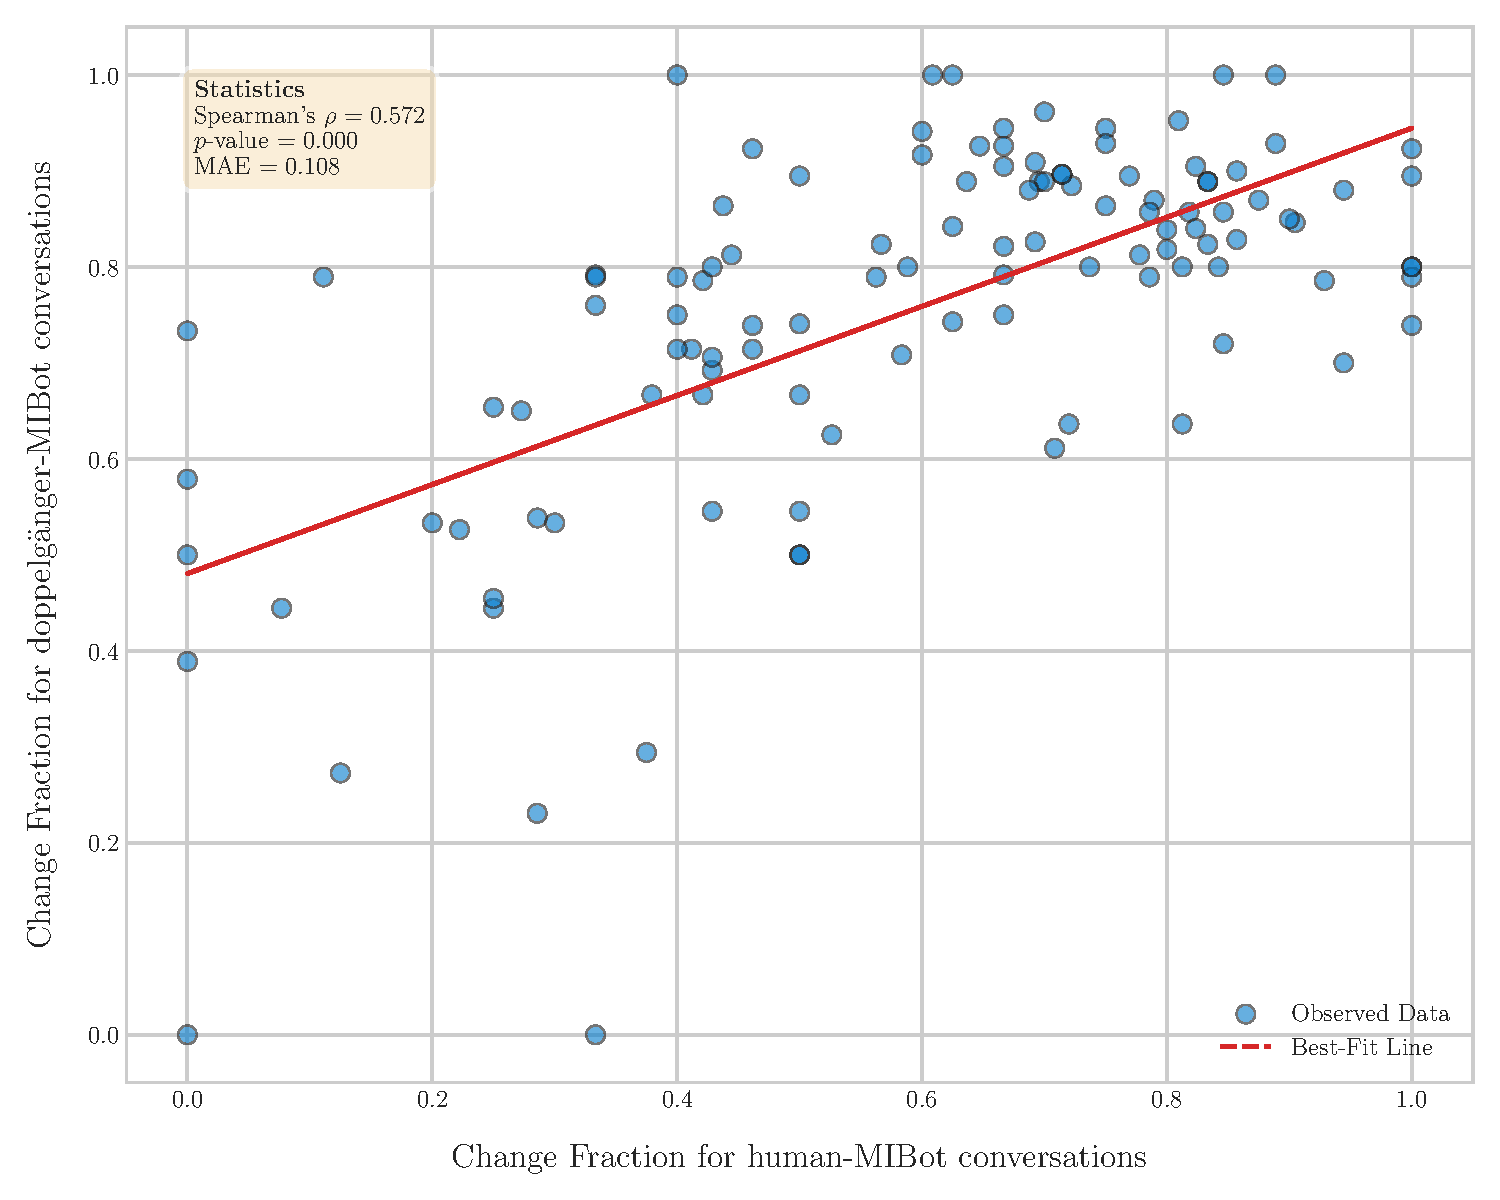
\includegraphics[width=0.7\textwidth]{fig/cf_doppelganger_human.pdf}
	\caption[Scatterplot of change fraction for humans and doppelgängers]{Scatter plot of change fraction for human--MIBot \textbf{(x-axis)} and doppelgänger--MIBot \textbf{(y-axis)} conversations.}
	\label{fig:cf_human_vs_doppel}
\end{figure}



\begin{figure}[ht!]
	\centering
	\begin{minipage}{0.8\textwidth}
		\centering
		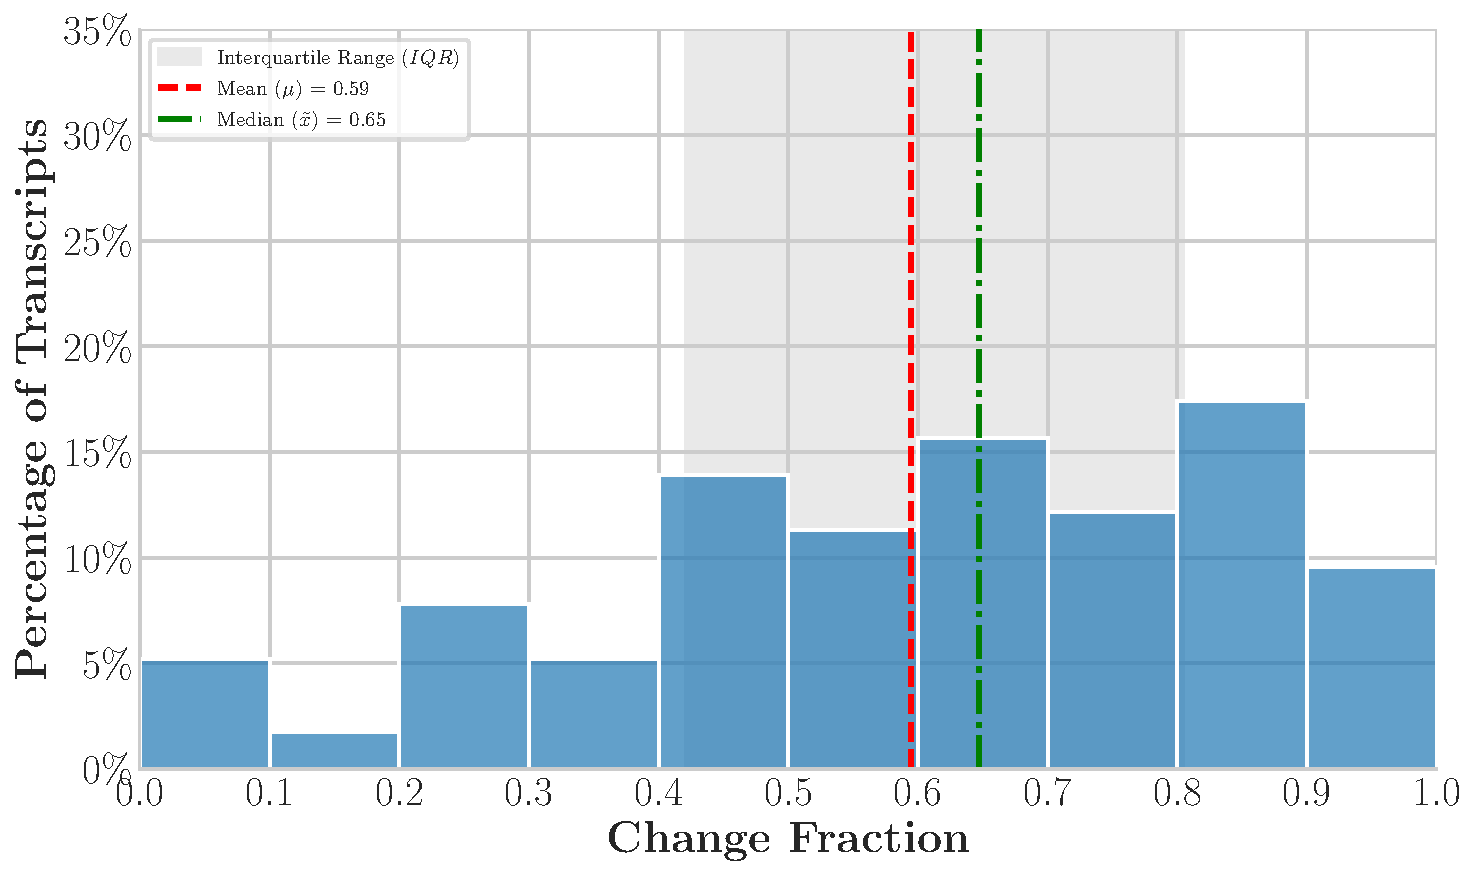
\includegraphics[width=\linewidth]{fig/change_frac_human_histogram.pdf}
		\subcaption{Change fraction for human--MIBot conversations}
	\end{minipage}\vfill
	\begin{minipage}{0.8\textwidth}
		\centering
		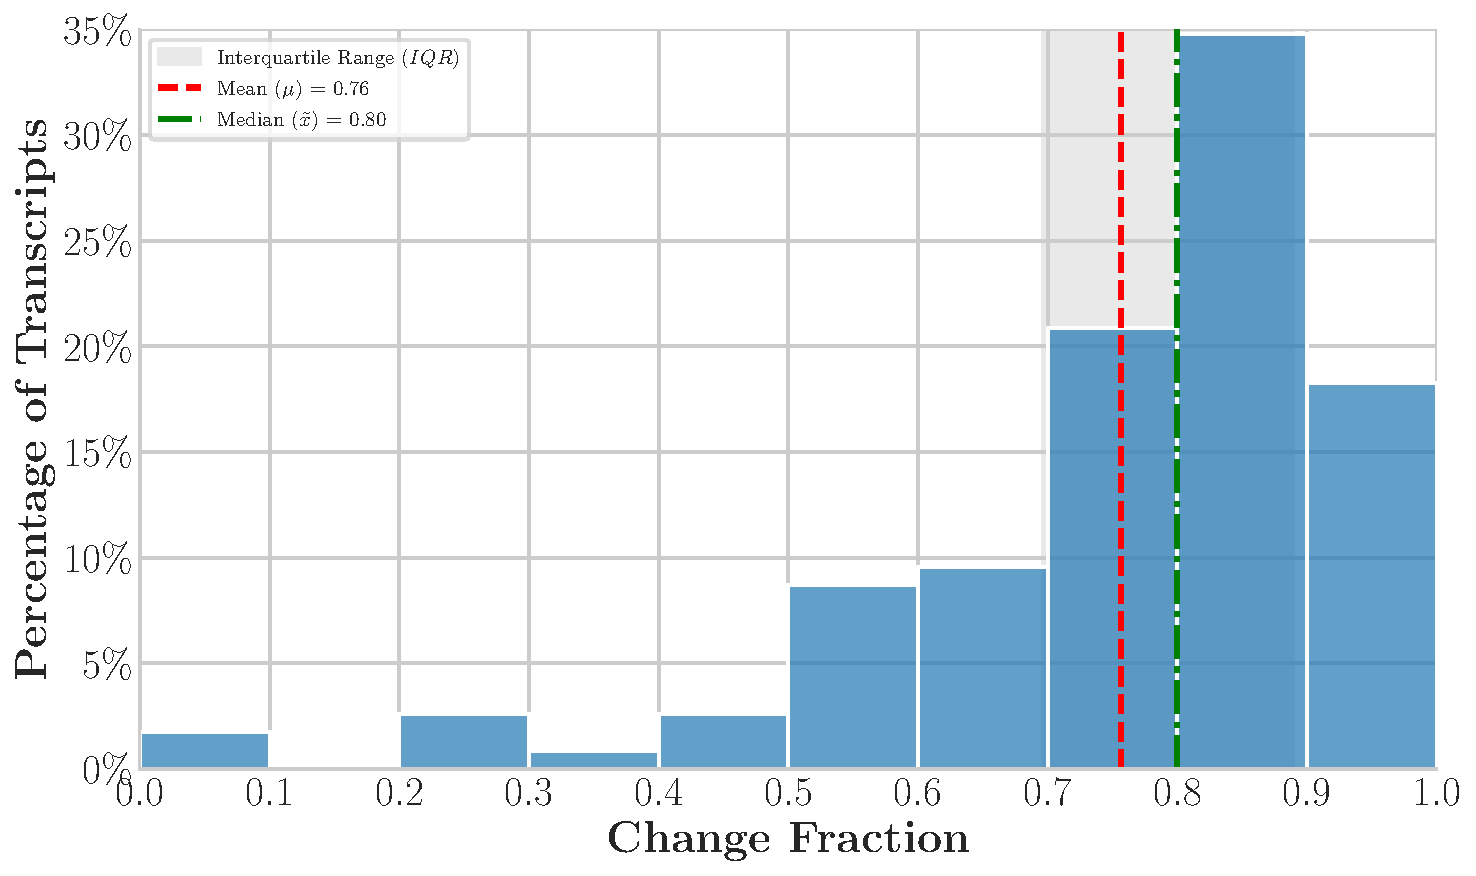
\includegraphics[width=\linewidth]{fig/change_frac_histogram.pdf}
		\subcaption{Change fraction for doppelgänger--MIBot conversations}
	\end{minipage}
	\caption[Distribution of change fraction (CF) for humans and doppelgängers]{Distribution of change fraction (CF) for \textbf{(a)} human--MIBot and \textbf{(b)} doppelgänger--MIBot conversations. Change fraction (CF) = \%CT$/100$. Doppelgängers tend to exhibit high CF compared to their human twins.}
	\label{fig:cf_comparison}
\end{figure}


\begin{table}[th!]
	\centering
	\begin{threeparttable}
		\begin{tabular}{@{}lcccc@{}}
			\toprule
			\textbf{}      & \textbf{}  & \textbf{Human}     & \textbf{Doppelgänger} & \textbf{Spearman's}  \\
			\textbf{Group} & \textbf{N} & \textbf{\%CT}      & \textbf{\%CT}         & \textbf{Correlation} \\
			\textbf{}      & \textbf{}  & \textbf{Mean (SD)} & \textbf{Mean (SD)}    & \textbf{($r_s$)}     \\
			\midrule
			Male           & 53         & 0.60 (0.27)        & 0.77 (0.14)           & 0.65\tnote{****}     \\
			Female         & 62         & 0.59 (0.25)        & 0.75 (0.22)           & 0.52\tnote{****}     \\
			\bottomrule
		\end{tabular}
		\begin{tablenotes}
			\item[****] \footnotesize $p < 0.0001$.
		\end{tablenotes}
	\end{threeparttable}
	\caption[Fidelity of doppelgänger's motivational language stratified by sex]{Fidelity of doppelgänger's motivational language stratified by sex. Fidelity is measured by the Spearman correlation between the percentage change talk (\%CT) of human participants and their corresponding doppelgängers.}
	\label{tab:doppelgänger-fidelity-sex}
\end{table}





\section{Synthetic Smokers' Sensitivity to Counselling Quality}


To assess the utility of synthetic smokers in testing and training applications, an experiment was conducted to determine if they are sensitive to the quality of counselling they receive.


\textbf{Rationale:} This experiment was designed to test whether synthetic smokers would exhibit differential responses when interacting with high-quality MI versus low-quality, confrontational counselling.

\subsection{Methodology}

\begin{enumerate}
	\item \textbf{Sampling:} Two participant groups (N=25 each) were created based on their actual change fraction (CF) in the MIBot study: a High-CF group (top 25th percentile) and a Low-CF group (bottom 25th percentile).

	\item \textbf{Doppelgänger Creation:} Doppelgängers were created for these 50 participants using the methodology described previously.

	\item \textbf{Counsellor Conditions:} These doppelgängers were exposed to two different automated counsellors:
	      \begin{itemize}
		      \item \textbf{Good MI Counsellor (MIBot v6.3A):} A high-quality, MI-adherent chatbot.

		      \item \textbf{Bad (Confrontational) Counsellor:} An LLM prompted to be directive, judgmental, and confrontational (see \Cref{app:doppelganger-prompts} for the full prompt).
	      \end{itemize}
\end{enumerate}

\subsection{Evaluation}
We measured the change fraction (CF), the change in confidence after a simulated week ($\Delta$Confidence), and the CARE score as reported by the doppelgängers.

\subsection{Results}

\begin{table}[ht!]
	\centering
	\begin{tabular}{@{}llccc@{}}
		\toprule
		\textbf{Counsellor}                    & \textbf{Participant Group} & \textbf{CF} & \textbf{$\Delta$Confidence} & \textbf{CARE} \\ \midrule
		\multirow{2}{*}{Good (MIBot 6.3A)}     & High-CF Doppelgängers      & 0.80        & 1.4                         & 49.8          \\
		                                       & Low-CF Doppelgängers       & 0.48        & 1.1                         & 47.8          \\ \midrule
		\multirow{2}{*}{Bad (Confrontational)} & High-CF Doppelgängers      & 0.68        & 1.1                         & 41.0          \\
		                                       & Low-CF Doppelgängers       & 0.22        & 0.5                         & 23.0          \\ \bottomrule
	\end{tabular}
	\caption[Effect of counselling quality on doppelgängers' motivational language]{Doppelgänger outcomes when interacting with good (MIBot 6.3A) vs. bad (confrontational) automated counsellors.}
	\label{tab:good-vs-bad-counselling}
\end{table}

The results, as detailed in Table 7.6, indicate that the synthetic smokers were sensitive to counselling quality. When interacting with the bad counsellor, outcomes were significantly worse across all metrics. The change fraction (CF) dropped markedly, particularly for the Low-CF group (from 0.48 to 0.22), suggesting increased resistance. The change in confidence was lower, and the CARE scores showed a pronounced difference (e.g., 23.0 vs. 47.8 for the Low-CF group).

These findings suggest that synthetic doppelgängers react in a predictable manner, responding negatively to poor-quality counselling. This sensitivity highlights their potential utility as evaluation and training tools.

\section{Conclusion}

This chapter detailed an advanced, data-driven approach to the development and validation of synthetic smokers, centred on the ``doppelgänger'' methodology. The experiments showed that installing pre-conversation readiness rulers was a key factor in aligning the doppelgänger's self-reported outcomes with those of their human counterparts. The conversational impact modelling and incremental attribute installation experiments yielded high correlations between synthetic and human data. Notably, the explicit installation of a participant's change fraction value led to the doppelgänger's conversational output correlating strongly with the human data (Spearman's $r_{s}=0.57$).

However, the process also revealed several challenges. For example, the correlation of CARE scores was negligible, and a population-level bias was observed, with doppelgängers generally exhibiting higher average change talk than humans.

The validation experiments demonstrated that doppelgängers are sensitive to the quality of motivational interviewing. They reacted differently to high-fidelity MI compared to confrontational counselling, showing reduced positive outcomes and lower perceived empathy scores when faced with poor therapeutic techniques. This sensitivity suggests the potential of synthetic smokers as a tool for the continued development and improvement of MIBot and for providing feedback to novice MI counsellors on their skills.